\onlyinsubfile{\setcounter{section}{5}}
\section{Extension: Estimating a lognormal distribution of returns}
\notinsubfile{\label{sec:lognorm}}

\par As I mentioned before, \cite{aflgdmlp20} document a persistent component to individual returns using the Norwegian population data. In fact, they include a graphic of the distribution of the estimated fixed effect in the return to net worth for individuals, which is clearly not uniformly distributed. For this reason, I rerun the estimation of my model under the assumption that returns are instead lognormally distributed across households. As we will see, the takeaways from my paper are robust to this change.

\subsection{Infinite horizon}

\par 

\begin{figure}[h]
    \centering
    \begin{minipage}{0.48\textwidth}
        \centering
        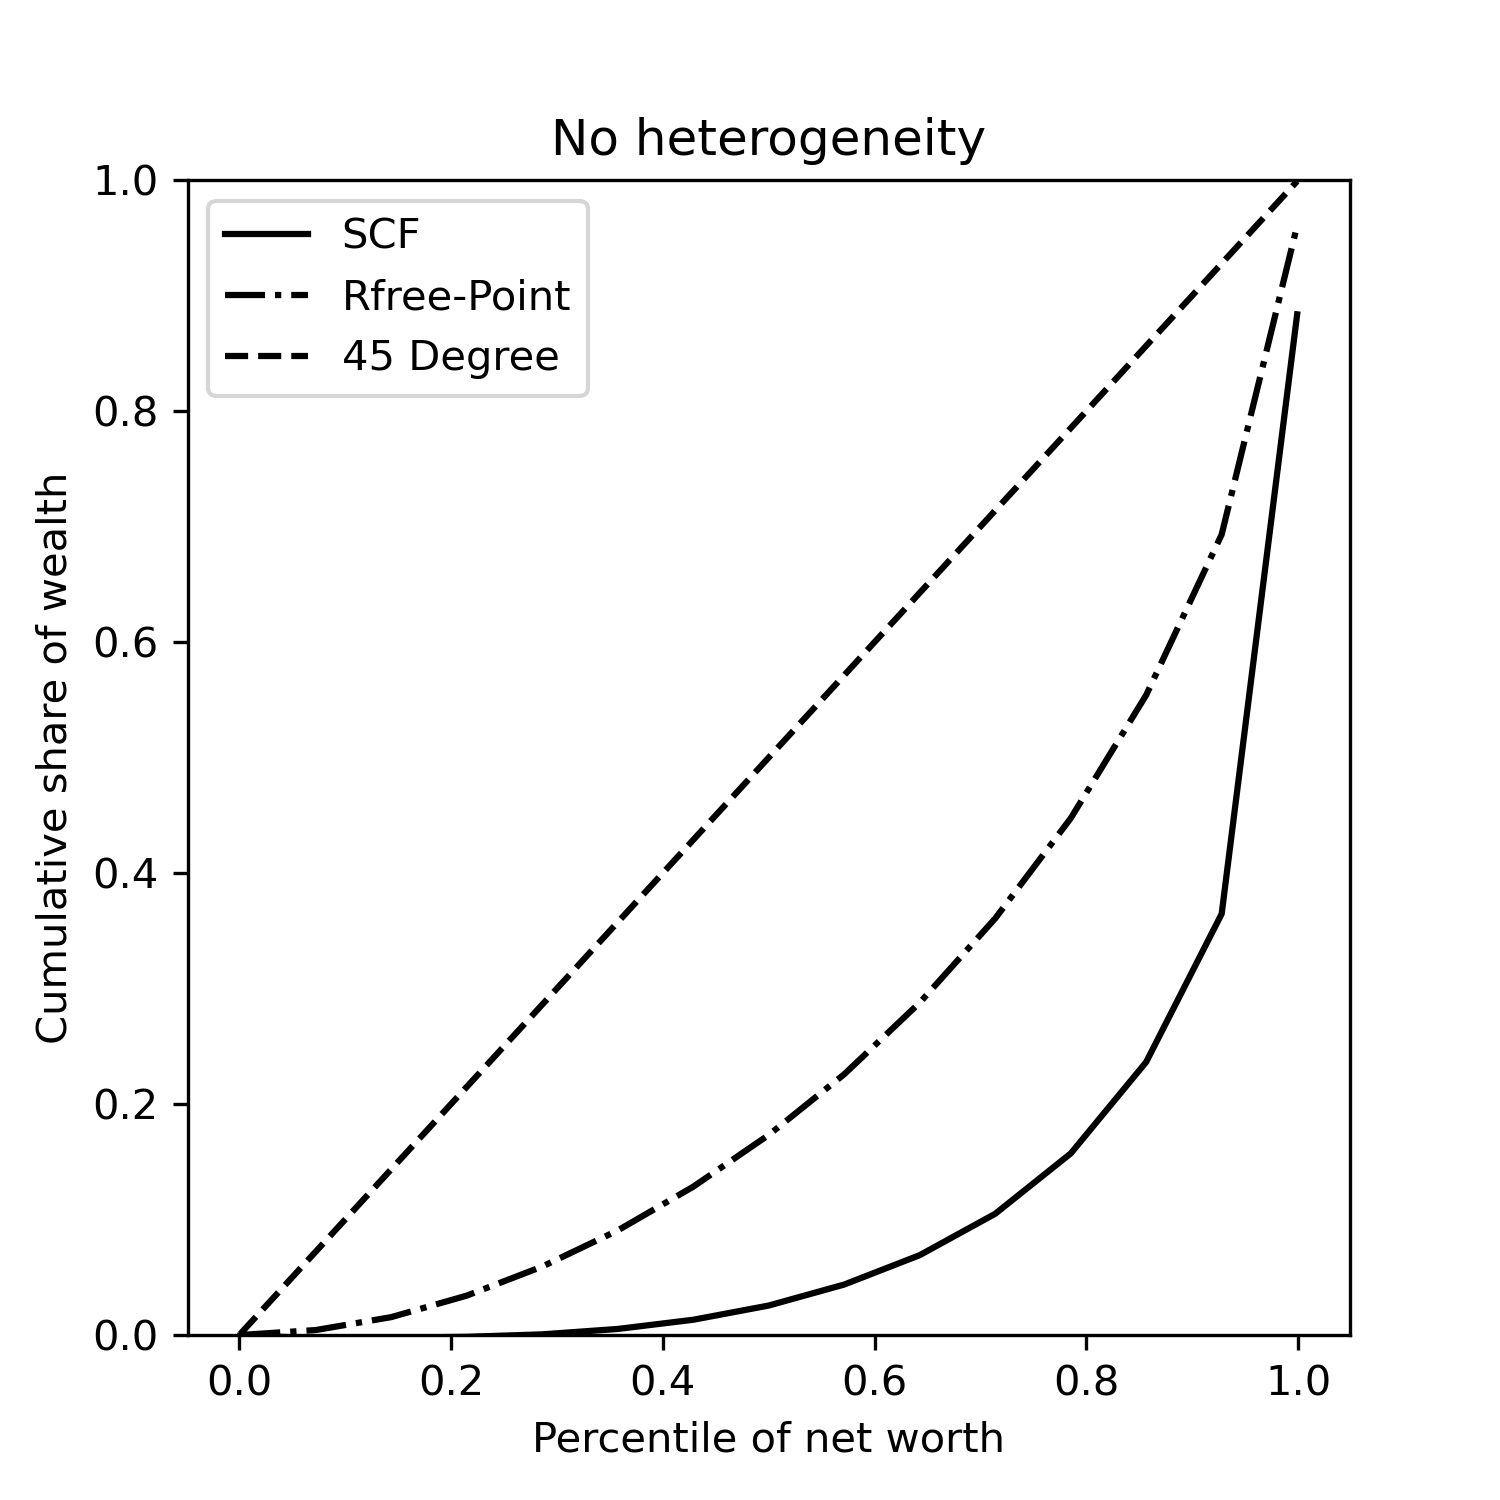
\includegraphics[width=\textwidth]{../Figures/Lognorm_PYrrPointNetWorth_2004Plot.png}
    \end{minipage}
    \hfill
    \begin{minipage}{0.48\textwidth}
        \centering
        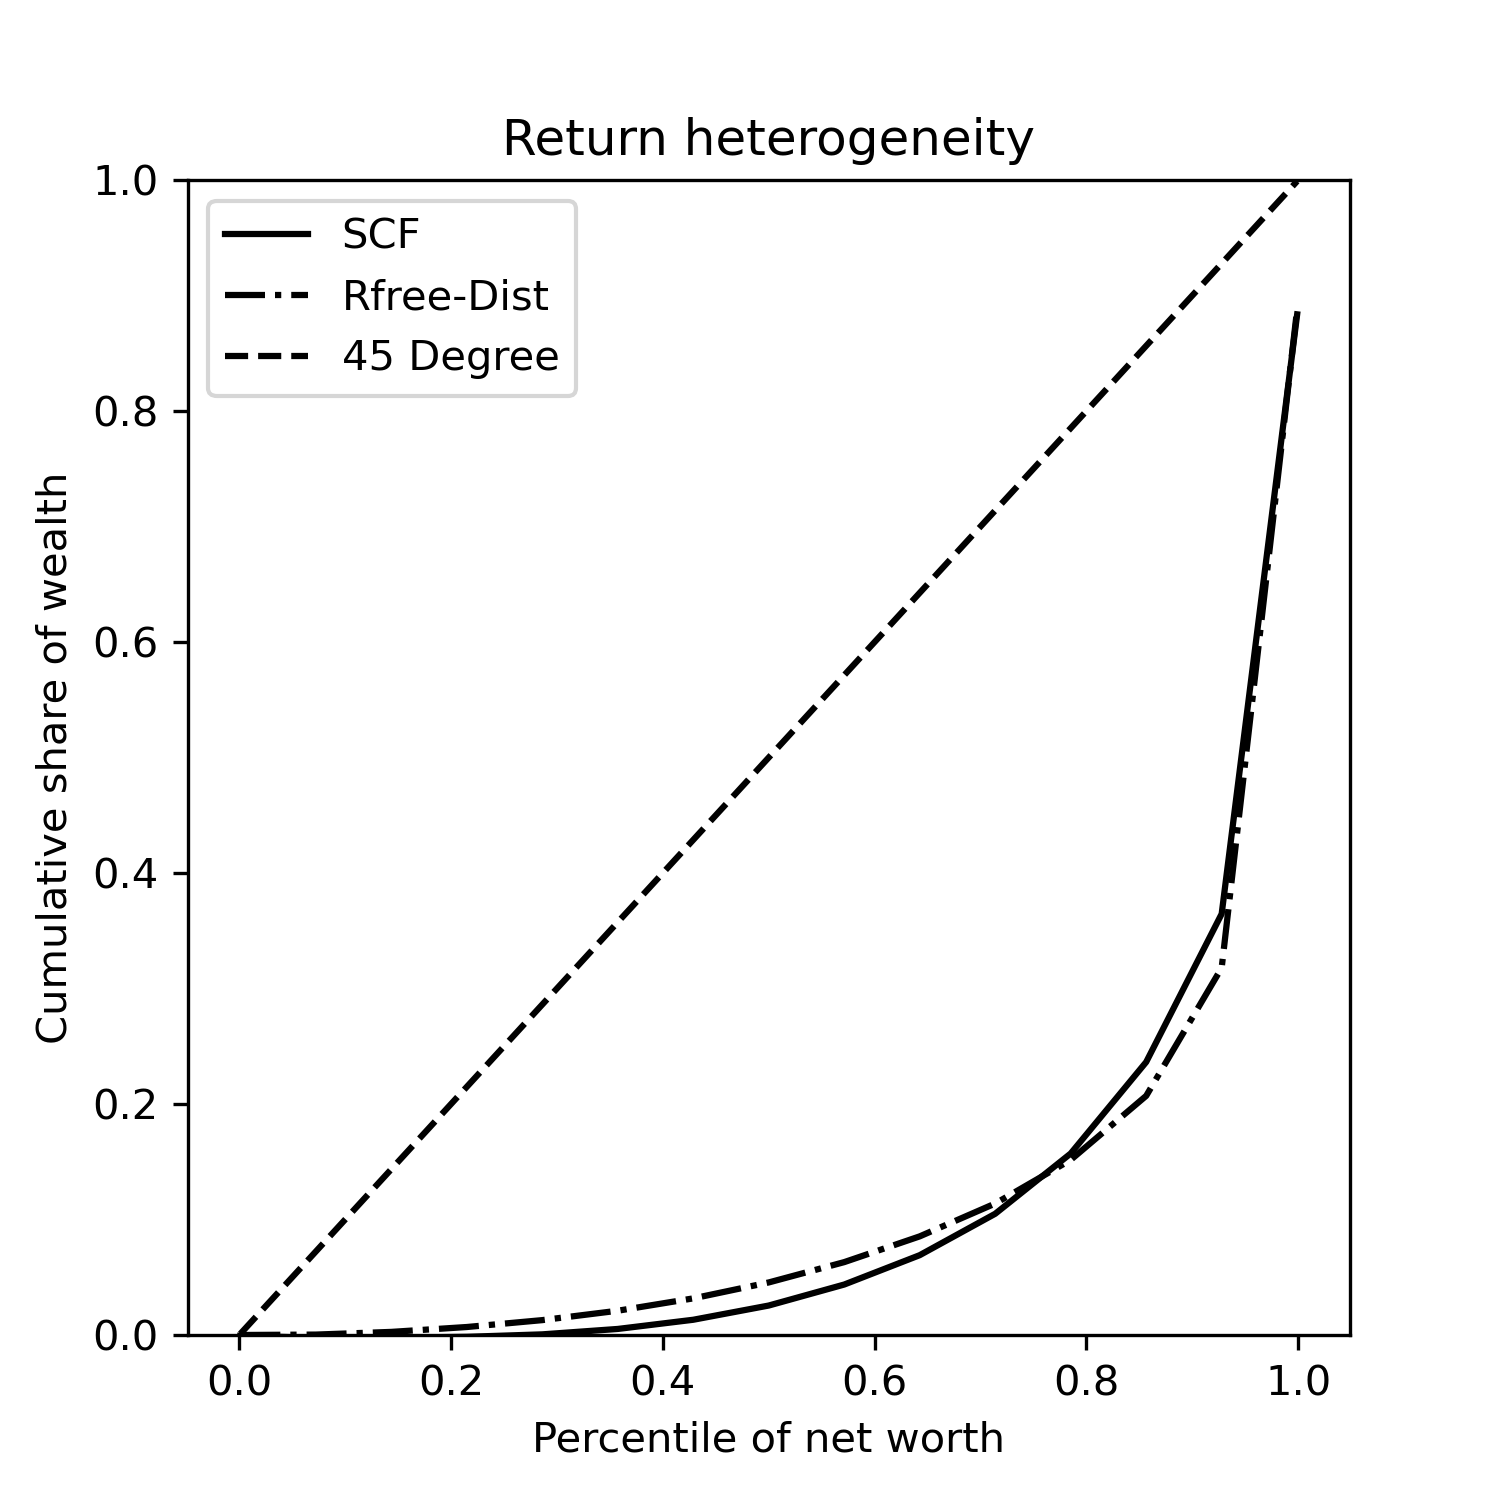
\includegraphics[width=\textwidth]{../Figures/Lognorm_PYrrDistNetWorth_2004Plot.png}
    \end{minipage}
    \caption{Comparison of R-Point and R-Dist Models .}
    \label{fig:PYLognorm} 
\end{figure}


\par


\par

\subsection{Life cycle dynamics}

\par 

\begin{figure}[h]
    \centering
    \begin{minipage}{0.48\textwidth}
        \centering
        \includegraphics[width=\textwidth]{../Figures/Lognorm_LCrrPointNetWorth_2004Plot.png}
    \end{minipage}
    \hfill
    \begin{minipage}{0.48\textwidth}
        \centering
        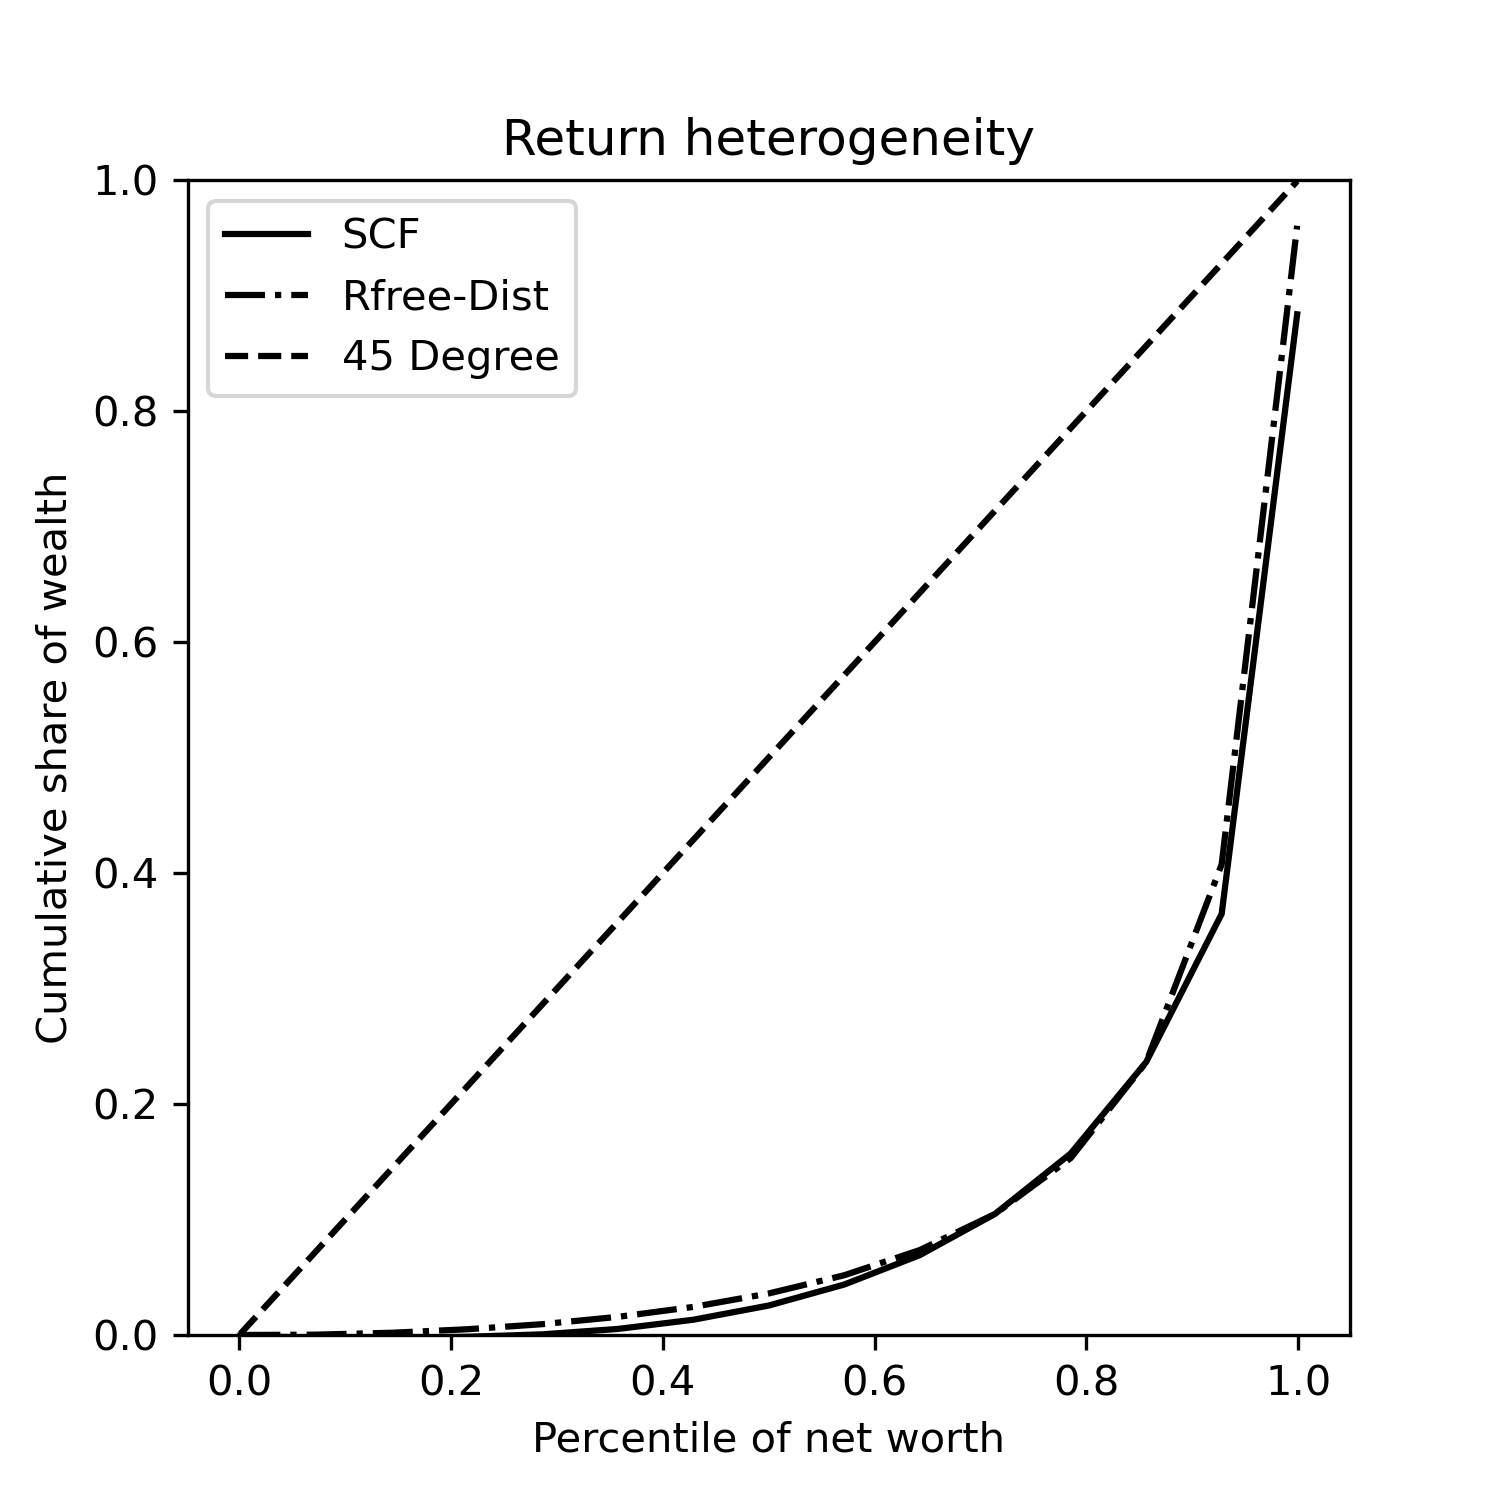
\includegraphics[width=\textwidth]{../Figures/Lognorm_LCrrDistNetWorth_2004Plot.png}
    \end{minipage}
    \caption{Comparison of R-Point and R-Dist Models in the Life-Cycle Setting.}
    \label{fig:LCLognorm} 
\end{figure}


\par


\subsubsection{Comparing the simulated wealth distributions}

\par

\begin{table}[htbp]
\centering
\caption{Wealth Distribution (Lognormal Returns)}
\label{tab:Lognorm_PY_LC_wealth_distribution_compare}
\small
\setlength{\tabcolsep}{10pt}
\renewcommand{\arraystretch}{1.15}
\resizebox{\textwidth}{!} \\
\hline
\textbf{Wealth share (data)} & -0.002 & 0.011 & 0.044 & 0.118 & 0.255 & 0.574 \\
\textbf{Wealth share (PY)}   &  0.006 & 0.021 & 0.044 & 0.088 & 0.225 & 0.616 \\
\textbf{Wealth share (LC)}   &  0.004 & 0.016 & 0.039 & 0.107 & 0.335 & 0.498 \\
\hline\hline
\end{tabular}%
}
\end{table}



\subsection{Untargeted moments}

\par 


\par

\begin{figure}[htbp]
\centering
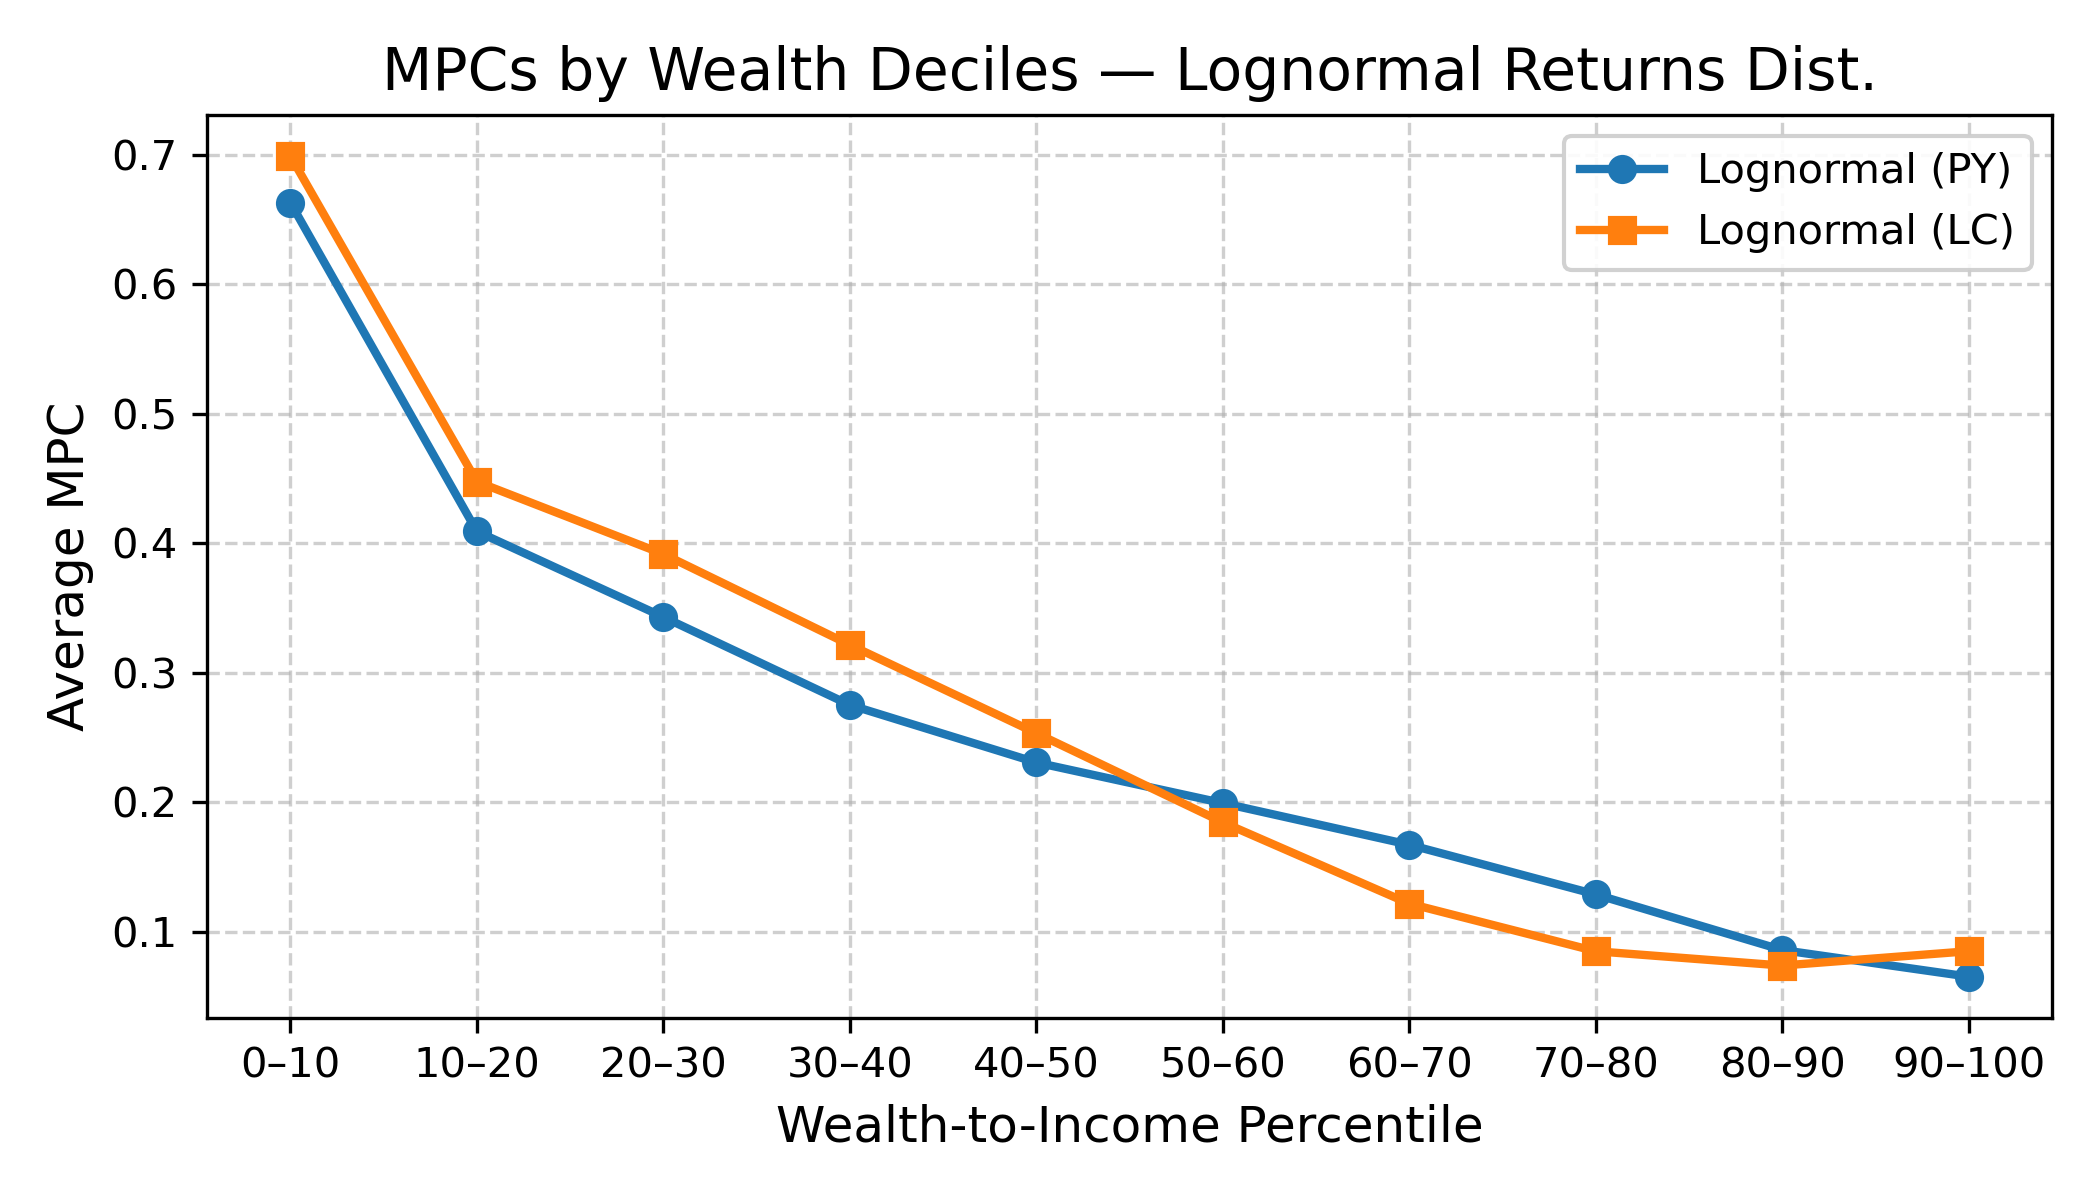
\includegraphics[width=0.8\textwidth]{Tables/Lognorm_PY_LC_MPC_by_WealthDecile_compare.png}
\label{fig:LognormPYLCMPCCompare}
\end{figure}


\par

\begin{figure}[htbp]
\centering
\includegraphics[width=0.8\textwidth]{Tables/Sim_Lorenz_by_age_Lognorm_LCrrPointNetWorth_2004.png}
\caption{Simulated Untargeted Moments without Heterogeneity (R-point).}
\label{fig:SimLorenzTarPoint}
\end{figure}

\begin{figure}[htbp]
\centering
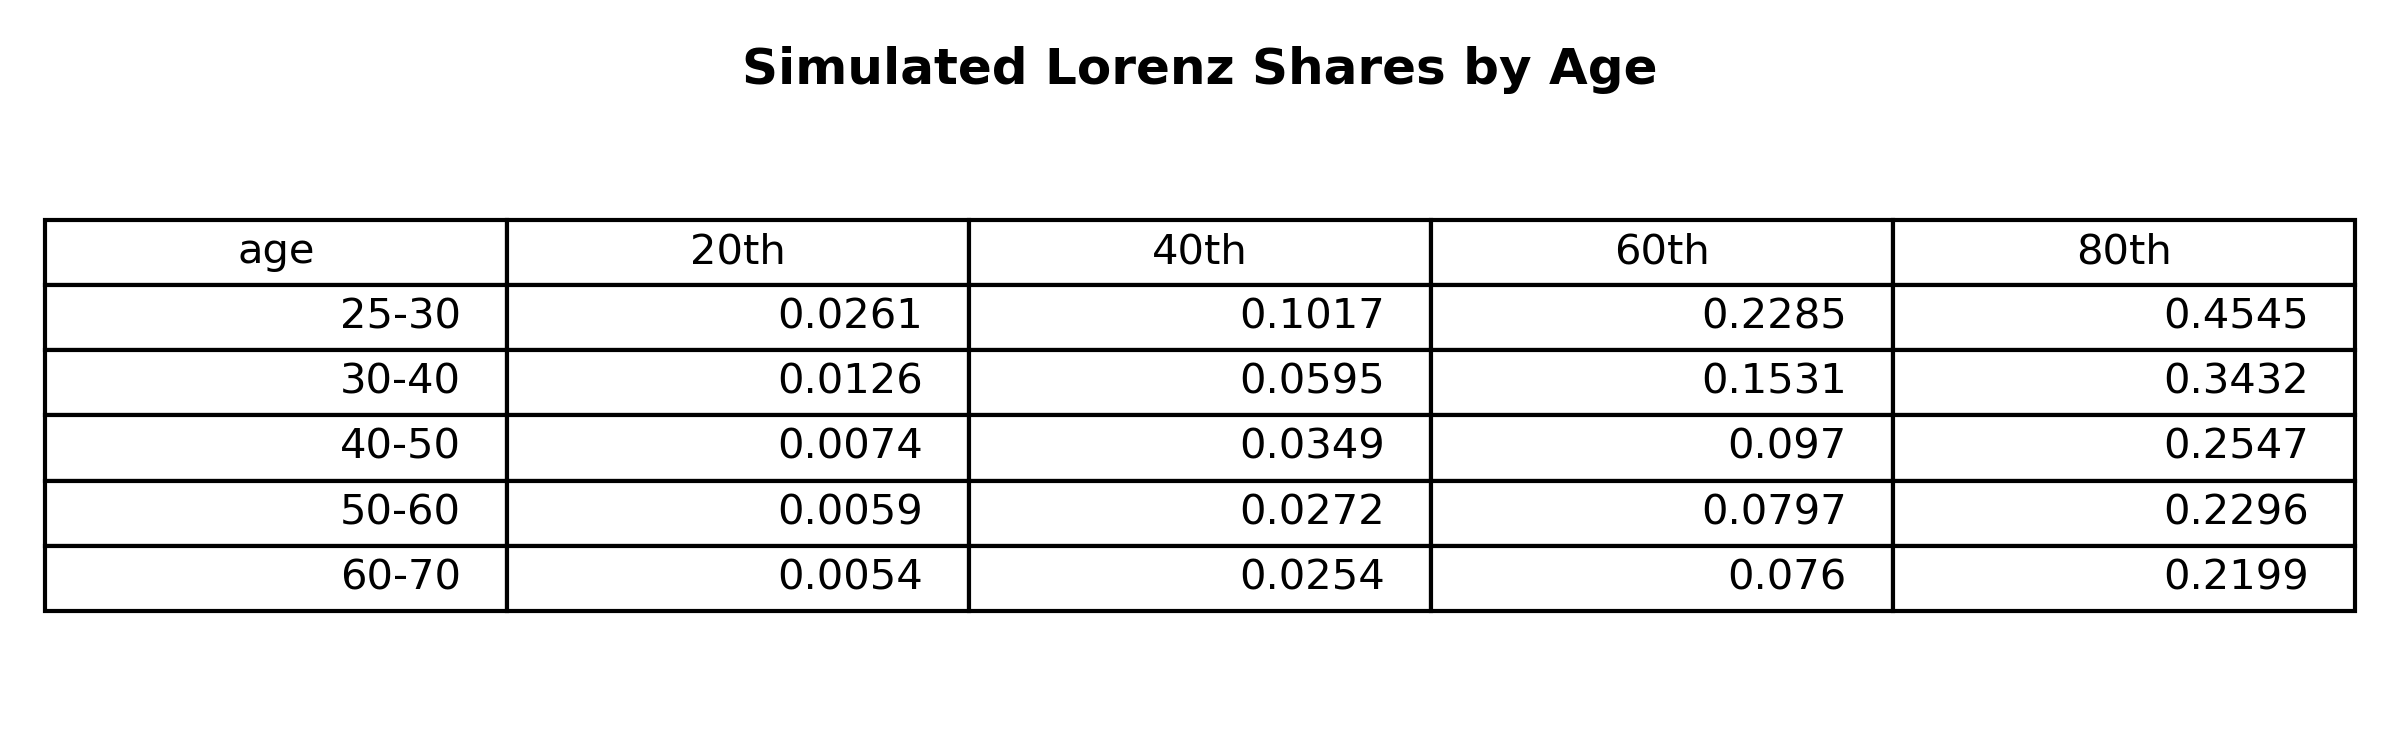
\includegraphics[width=0.8\textwidth]{Tables/Sim_Lorenz_by_age_Lognorm_LCrrDistNetWorth_2004.png}
\caption{Simulated Untargeted Moments with Heterogeneity (R-dist).}
\label{fig:SimLorenzTarDist}
\end{figure}

\subsection{Tax implications}

\par 

\begin{table}[!htbp]
\centering
\caption{Expected Welfare Gains from Tax Reform (Lognormal Returns)}
\label{tab:ce_welfare_tax_lognorm}
\begin{threeparttable}
\begin{tabular}{lcc}
\toprule
& \textbf{Infinite horizon} & \textbf{Life-cycle} \\
\midrule
WT vs CIT       & 0.22\% & 0.18\% \\
WT vs Original  & 0.78\% & 0.36\% \\
CIT vs Original & 0.56\% & 0.18\% \\
\bottomrule
\end{tabular}
\begin{tablenotes}[flushleft]
\footnotesize
\item Notes: Entries are consumption-equivalent (CE) welfare gains, $\Delta$, expressed as percent changes under the assumption that individual returns follow a lognormal distribution across households. 
\end{tablenotes}
\end{threeparttable}
\end{table}


\par

% Requires: \usepackage{booktabs,threeparttable}
\begin{table}[!htbp]
\centering
\caption{Per-Type Welfare Gain and Baseline Return (WT vs CIT, Lognormal Returns)}
\label{tab:ce_per_type_wt_vs_cit_lognorm}
\begin{threeparttable}
\begin{tabular}{lccccccc}
\toprule
& \textbf{Type 1} & \textbf{Type 2} & \textbf{Type 3} & \textbf{Type 4} & \textbf{Type 5} & \textbf{Type 6} & \textbf{Type 7} \\
\midrule
Baseline $R$ (gross) & 0.976 & 1.001 & 1.014 & 1.026 & 1.038 & 1.053 & 1.079 \\
CE $\Delta$ (WT vs CIT, \%) & 0.267\% & 0.342\% & 0.329\% & 0.317\% & 0.308\% & 0.304\% & -0.326\% \\
\bottomrule
\end{tabular}
\begin{tablenotes}[flushleft]
\footnotesize
\item Notes: CE entries are per-type consumption-equivalent welfare gains (pmv-weighted within type), expressed as percent. Positive values favor the wealth tax over the capital income tax for that return type. Baseline $R$ values are pre-tax gross returns (low $\rightarrow$ high) under the lognormal returns specification.
\end{tablenotes}
\end{threeparttable}
\end{table}


% Requires: \usepackage{booktabs, threeparttable, multirow, graphicx}

\begin{table}[!htbp]
\centering
\caption{Per-Education Per-Type Welfare Gain and Baseline Return (WT vs CIT, Lognormal Returns)}
\label{tab:ce_per_type_wt_vs_cit_lc_lognorm}
\begin{threeparttable}

\begin{minipage}{\linewidth}
\centering
\resizebox{\linewidth}{!}{%
\begin{tabular}{llccccccc}
\toprule
\multicolumn{2}{c}{} & \textbf{Type 1} & \textbf{Type 2} & \textbf{Type 3} & \textbf{Type 4} & \textbf{Type 5} & \textbf{Type 6} & \textbf{Type 7} \\
\midrule
\multirow{2}{*}{NoHS}
  & Baseline $R$ (gross)        & 0.9363 & 0.9711 & 0.9910 & 1.0084 & 1.0260 & 1.0471 & 1.0865 \\
  & CE $\Delta$ (WT vs CIT, \%)  & 0.132\% & 0.176\% & 0.225\% & 0.275\% & 0.335\% & 0.292\% & -0.114\% \\
\midrule
\multirow{2}{*}{HS}
  & Baseline $R$ (gross)        & 0.9363 & 0.9711 & 0.9910 & 1.0084 & 1.0260 & 1.0471 & 1.0865 \\
  & CE $\Delta$ (WT vs CIT, \%)  & 0.131\% & 0.177\% & 0.229\% & 0.283\% & 0.332\% & 0.250\% & -0.098\% \\
\midrule
\multirow{2}{*}{College}
  & Baseline $R$ (gross)        & 0.9363 & 0.9711 & 0.9910 & 1.0084 & 1.0260 & 1.0471 & 1.0865 \\
  & CE $\Delta$ (WT vs CIT, \%)  & 0.131\% & 0.177\% & 0.228\% & 0.276\% & 0.311\% & 0.218\% & -0.096\% \\
\bottomrule
\end{tabular}%
} % end resizebox
\end{minipage}

\begin{tablenotes}[flushleft]
  \footnotesize
\item 
  Notes: CE entries are consumption-equivalent welfare gains (pmv-weighted within type), \\
  expressed as percent. Positive values favor wealth taxation over capital income taxation \\
  for that return type. Baseline $R$ are pre-tax gross returns by type (low $\rightarrow$ high)
  at $t=0$ \\ under the lognormal returns specification. 
\end{tablenotes}
\end{threeparttable}
\end{table}



\par